 \documentclass[sigconf]{acmart}

\usepackage{hyperref}

%\usepackage{endfloat}
%\renewcommand{\efloatseparator}{\mbox{}} % no new page between figures

\usepackage{booktabs} % For formal tables

\settopmatter{printacmref=false} % Removes citation information below abstract
\renewcommand\footnotetextcopyrightpermission[1]{} % removes footnote with conference information in first column
\pagestyle{plain} % removes running headers


\begin{document}
\title{Big Data Analytics, Data Mining, and Public Health Informatics: 
Using Data Mining of Social Media to Track Epidemics}
\author{Sean M. Shiverick}
% \orcid{1234-5678-9012}
\affiliation{%
  \institution{Indiana University-Bloomington}
}
\email{smshiver@indiana.edu}

\begin{abstract}

Data mining of internet search queries and social media for influenza related keywords 
has been used to track seasonal influenza and correlates highly with official reports 
of `infuenza-like-illness' (ILI). Efforts to monitor epidemics using big data analytics 
can provide early detection that supplements existing systems of disease surveillance. 
A review of the literature shows that data extracted from social media has applications 
for public health informatics. Prediction models based on social media work best in 
areas with a high degree of internet access.  

\end{abstract}

\keywords{i523, HID335, Data Mining, Social Media, Public Health Informatics}

\maketitle

\section{Introduction}

In the information age, \textit{Big Data} offers great promise to fuel innovation, 
generate new revenue streams, and transform society \cite{gupta15}. Can the 
potential of big data be harnessed for the greater good, to prevent disease 
and improve health? Seasonal influenza epidemics are a major public health concern, 
resulting each year in an estimated 250,000 to 500,000 deaths worldwide 
\cite{who16}. This paper explores big data in public health informatics, 
specifically reviewing research on data mining to track epidemics and the spread 
of contagious disease \cite{hay13}. Can these approaches be extended to monitor 
other epidemics such as the opioid crisis in North America? \cite{smith16}
Epidemic spreading is a complex phenomenon based on contact networks between 
individuals and distributed by transportation networks \cite{Colizza06}. Some 
questions remain as to whether prediction models based on social networking 
platforms can be generalized to other epidemics at future points in time. 
Limitations of using social media data to predict epidemics are discussed.


\subsection{Public Health Informatics}

The field of Health Informatics is generating huge amounts of data at a rapid pace,
from MRI imaging data, electronic medical records (EMRs), clinical research data, to
population-level data. This review focuses on population data from search queries and 
social media to provide insights about epidemics and pandemics \cite{hay13, herland14}. 
Big data is an ambiguous term that lacks a single unified definition, but is often 
described in terms of {\it Volume, Velocity, Variety, Veracity, and Value}
\cite{demchenko12}. Trying to track an epidemic in real-time from multitudes of 
incoming web searches and posts involves a high volume of data coming in at high 
velocity \cite{lamb13, paul14}. In order to be of any use, diverse and often messy 
raw data has to be sifted through and effectively organized for further analysis. 
The issue of Veracity raises the questions of how reliable social media data are for 
predicting real life events. What is the relationship between social media data to 
biological events such as the spreading of contagion and disease? The question of 
Value evaluates the quality of the data as it pertains to intended outcomes, such 
as limiting the spread of contagion and disease prevention. There are legitimate 
concerns about the quality of data obtained from the internet; however, the 
literature suggests that mining information from social media can produce valuable 
data. An important challenge for making sense of big data is developing analytic 
tools adequate to handle large volumes of data in real time.

\subsection{Data Mining Social Media}

Health Informatics research is considered from two levels: where the data is 
collected, and the research questions being addressed. Research on social media 
can yield data on a range of issues related to public health, including: 
spatiotemporal information of disease outbreaks, real-time tracking of infectious 
diseases, global distributions of various diseases, and search queries on medical 
questions that people might have \cite{herland14}. The questions of interest in the 
current review are: \textit{Can search query data be used to accurately track epidemics 
in real-time?} and, \textit{can Twitter data be used to monitor epidemics across 
different regions?} The general idea is that increasing search query or social 
media activity is associated with an increasing interest in a given health topic. 
A limitation of social media data is that, although it has high Volume, Velocity, 
and Variety, it can be unreliable, resulting in both low Veracity and Value 
\cite{hay13, lazer14}. A review of the literature shows how useful data can be 
extracted by data mining and analytic techniques. 

\subsection{Using Search Queries to Track Epidemics}

\subsubsection{Tracking Epidemics Using {\itshape Google} Search Terms in the U.S.}

Seasonal influenza is an acute viral infection that spreads easily from person to 
person, circulates across regions, affecting people of every age. Traditional flu 
monitoring estimates from the U.S. Center of Disease Control and Prevention (CDC) 
based on physician reports of patients with ``{\it influenza-like illness}'' (ILI) are 
released weekly \cite{cdc17}, but generally with a one to two week delay. In an effort 
to improve on early detection of season influenza, a team of researchers developed an 
automated method to analyze Google search queries to track ILI terms from historical 
logs between 2003 and 2008, using 50 million most popular searches, and CDC historical 
data \cite{ginsburg09}. The {\it Google Flu Trends} (GFT, https://www.google.org/flutrends)
model sought to find the probability that a given search query is related to an ILI of a 
patient visiting a physician in the same region. GFT used a feature selection method to 
narrow the 50 million most popular search queries, aggregrated from historical, down to 
45. These top 45 search queries yielded the highest estimates during cross validation 
and were connected with influenza symptoms, complications, remedies, consistent with 
searches by individuals with influenza. Estimates of the current level of weekly 
influenza were based on the correlation of the relative frequency of search queries 
and the percentage of physician visits with patients presenting influenza-like symptoms. 
The GFT model was trained on 128 points of the mid-Atlantic region of the U.S. (e.g., 
New York, New Jersey, Pennsylvania) between 2004 to 2007 with a correlation of 0.85, 
and validated on 42 points between 2007 to 2008, with a correlation of 0.96 (see Figure 1). 
The final model, for all regions in the U.S., generated correlation estimates ranging 
from 0.92 to 0.99 over 42 points. Thus, analyzing high volume Google search queries 
estimated ILI percentages across several regions in the U.S. about 1 to 2 weeks 
earlier than official CDC ILI reports. Such efforts at early detection can help 
physicians and health care professional anticipate and prepare for the outbreak 
of influenza epidemics and pandemics. 

\begin{figure}
  \centering
  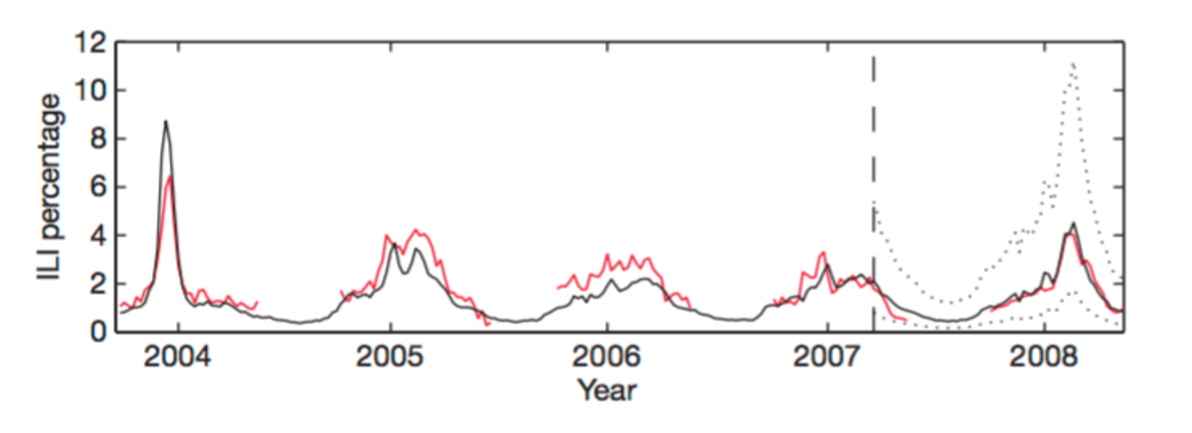
\includegraphics[width=0.5\textwidth]{images/Figure1.pdf}
  \caption{Comparison of GFT model estimates (black) for mid-Atlantic region of U.S. 
  (NY, NJ, PA) against CDC-reported ILI percentages (red) between 2004 to 2008 
  \cite{ginsburg09}} 
  \label{fig:Figure1} 
\end{figure}

\subsubsection{Tracking H1N1 Epidemic Using {\itshape Baidu} Queries in China}

Researchers in China monitored influenza activity by comparing internet search query 
data from {\it Baidu} (https://www.baidu.com) to influenza case counts from the Chinese 
Ministry of Health (MOH) between 2009 to 2012 during the H1N1 epidemic \cite{yuan13}. 
The study consisted of four parts: (i) Selecting keyword terms related to influenza, (ii) 
Filtering keywords unrelated to flu epidemics, (iii) Defining weights and composite search 
index, and (iv) Fitting a regression model with keyword index to influenza case data. In the 
process of filtering, only 40 of 94 keywords were correlated with the case data, and only 8 
of these 40 keywords were used as the optimal set in the composite search index. As expected,
the search index captured seasonal variation of influenza epidemics in the Winter and Spring,
indicating a good predictor for tracking influenza activity in China (see Figure 2). The 
regression model accounted for 95 percent of the variability in influenza case data (ICD), 
and the model was validated for a test period in 2012. The mean absolute percent error rate 
of prediction over an eight month period in 2012 was 10.6 (see Table 1). This research yields 
additional evidence that novel approaches using big data can provide early indicators of 
epidemic activity that supplement official public health information sources, rather than 
replacing them. A limitation acknowledged by the authors is the relatively small initial 
number of keyword search terms used compared to the Google Flu Trends (GFT) project 
\cite{ginsburg09}. Another limitation of using search query data is that, although the 
keywords selected in this model performed well at capturing temporal trends in the H1N1 
epidemic, the same keywords may not reflect the trend of an influenza epidemic at a future 
time. The authors also noted the lack of internet access in rural areas, which underscores 
the fact that effective tracking of epidemics based on search queries relies on internet 
access. Furthermore, caution should be used in evaluating correlational data, as causation 
cannot be inferred from correlation.

\begin{figure}
  \centering
  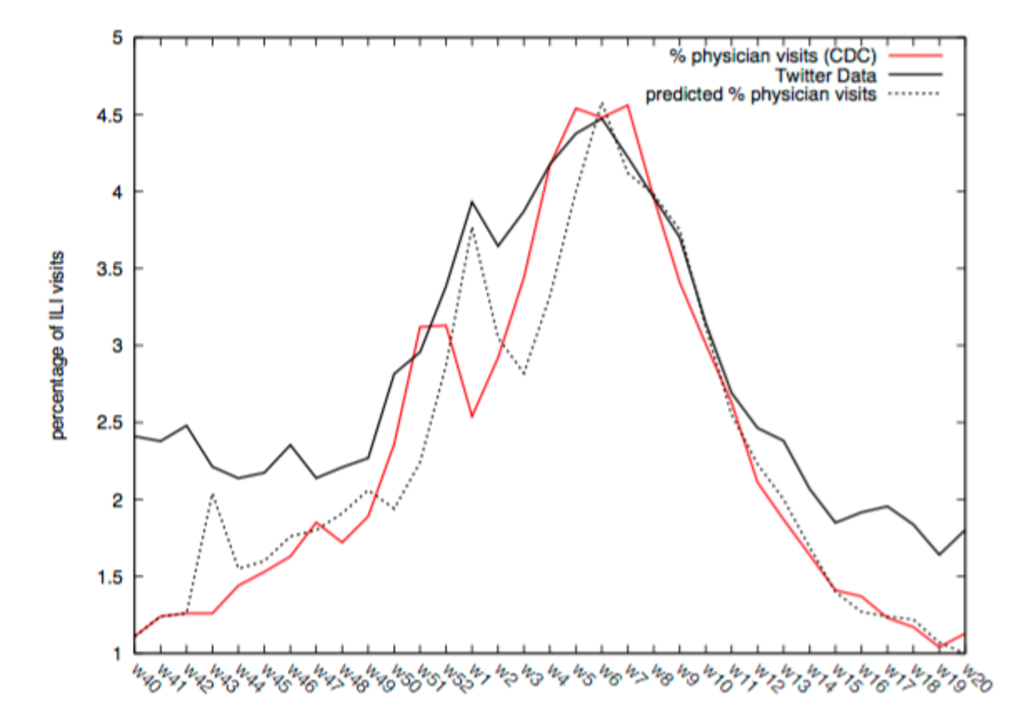
\includegraphics[width=0.5\textwidth]{images/Figure2.pdf}
  \caption{Plot of influenza cases, fitted values and prediction based on model \cite{yuan13}} 
  \label{fig:Figure2} 
\end{figure}

\begin{table*}
  \caption{Predicted values, errors, and mean absolute percent error of prediction based 
  on Baidu search queries in China for eight consecutive months (January to August 2012) 
  \cite{yuan13}}
  \label{tab:freq}
  \begin{tabular}{ccccc}
    \toprule
     Month&Actual values& Predicted Values& Absolute Error& Percent absolute error\\
    \midrule
    01-2012& 10045& 10230& 184& 1.8\\
    02-2012& 17421& 14578& 2843& 16.3\\
    03-2012& 21652& 18429& 3196& 14.8\\
    04-2012& 10707& 11785& 1078& 10.1\\
    05-2012& 8520& 8618& 98& 1.2\\
    06-2012& 6195& 6621& 426& 6.9\\
    07-2012& 6738& 5240& 1498& 22.2\\
    08-2012& 6793& 5983& 810& 11.9\\
    \bottomrule
  \end{tabular}
\end{table*}


\subsection{Using {\itshape Twitter} API Data to Track Epidemics}

Twitter is a free online social networking and micro-blogging service, where users can send 
and read messages of 140 characters (i.e., {\it ``tweets''}). As of 2017, Twitter has more 
than 320 million monthly active users (67 million in U.S.), with an estimated 500 million 
tweets posted per day (https://about.twitter.com). Twitter users share their perspectives and
reactions on a wide range of topics, approximately 80 percent from handheld mobile devices, 
acting as ``sensors'' of events in real time \cite{achrekar12}. The Twitter stream provides 
a rich data source for tracking or forecasting general sentiment, political attitudes, 
linguistic variation, detecting earthquakes, and disease surveillance. The large volume of 
users provides a high likelihood that ILI epidemic information is posted; however, Twitter 
post data is noisy and perhaps unreliable insofar as it can be difficult to differentiate 
posts about the flu based on instances of concerned awareness ({\it ``I am worried about 
the swine flu epidemic!''}), versus actual infection ({\it ``Robbie might have swine flu. 
I am worried.''})\cite{lamb13}. Despite the noise in Twitter data from much useless chatter, 
useful information be obtained from mining data in the Twitter stream. 


\subsubsection{Using Twitter to Track Disease Activity and Public Concern in the 
U.S. during the H1N1 Pandemic.}

In a 2011 study, researchers searched through post data from Twitter`s streaming API 
during the H1N1 epidemic (October 2009 to May 2010) across spatiotemporal areas of the 
U.S. to predict weekly ILI levels \cite{signorini11}. Tweets were sifted according to 
keywords related to H1N1 (e.g., {\it ``flu'', ``swine'', ``influenza''}) and additional 
terms about vaccines, side effects, and/or vaccine shortages. The first data set consisted 
of 951,697 tweets containing influenza related keywords from 334,840,972 tweets extracted 
between April to June 2009 (results were reported as a percentage of observed tweets). 
These tweets represent just over 1 percent of the sample tweet volume, and this percentage 
declined rapidly over time as the number of reported H1N1 cases increased. In the U.S. 
surveillance programs track reported influenza-like illness (ILI) seasonally, from October 
to May, monitoring the total number of patients seen along with the number with ILIs 
reported. Quantitative estimates of ILI values based on the Twitter stream were analyzed 
using support vector regression (SVR) and leave-one-out cross-validation to test model 
accuracy. Figure 3 shows the weekly ILI values nationwide reported by the CDC (green line)
and estimated using a model trained on roughly 1 million influenza-related Tweets (red line)
obtained between October, 2009 to May, 2010. The red line shows output from a leave one out 
cross validation based on SVM estimator. Point estimates of national ILI values produced 
by the system were good with an average error of 0.28 percent. A regional model, based on 
significantly fewer tweets, approximated the epidemic curve for CDC region 2 (New York, 
New Jersey) as reported by the ILI data, but the estimate was less precise with an average
error of 0.37 percent. In terms of public interest, Twitter users` interest in antiviral 
drugs dropped, as official disease reports indicated most influenza cases were relatively 
mild, even as the number of cases was increasing. In addition, interest in hand hygiene 
and face masks was associated with public health messages from CDC. A limitation of the 
study is that only a limited number of search terms and one prediction method was used. 
An important question is whether the results could be improved using broader search terms 
and other prediction models. 

\begin{figure}
  \centering
  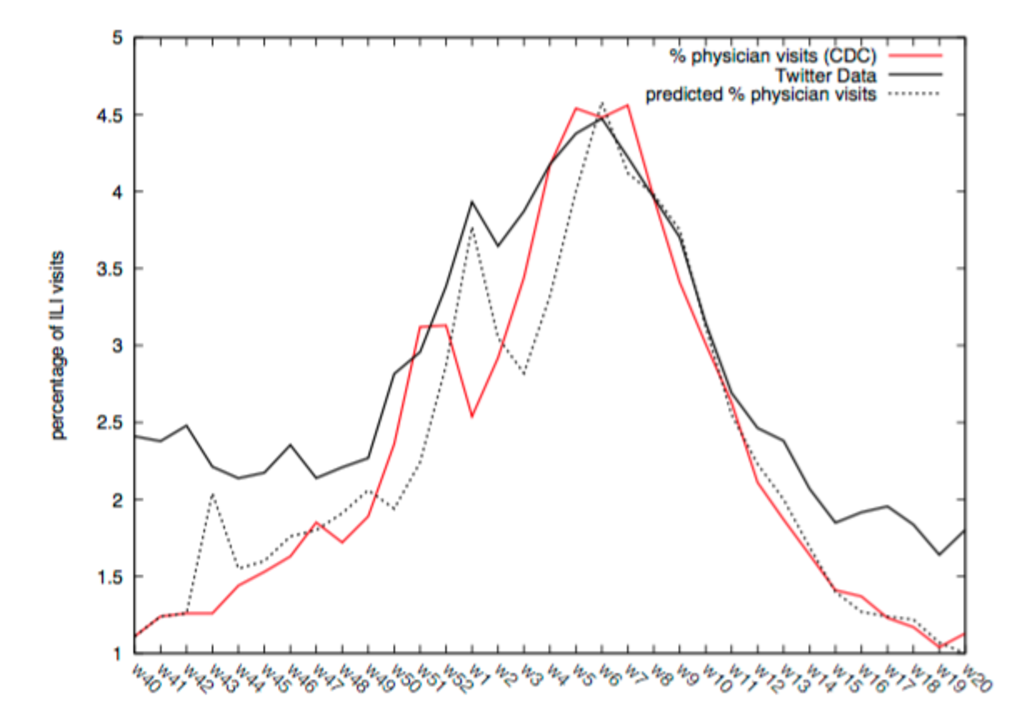
\includegraphics[width=0.5\textwidth]{images/Figure3.pdf}
  \caption{Weekly CDC reported (green) and Twitter estimated (red) ILI percent 
  Nationwide (U.S., 2009 to 2010) \cite{signorini11}} 
  \label{fig:Figure3} 
\end{figure}


\subsubsection{Twitter Improves Seasonal Influenza Prediction}

In a 2012 study, researchers implemented a system using an online social network (OSN)
Crawler bot to retrieve tweets by keywords (e.g., {\it ``flu'', ``H1N1'', ``swine flu''}), 
geospatial location, relative keyword frequency, and CDC ILI reports \cite{achrekar12}. 
The {\it Social Network Enabled Flu Trends} (SNEFT) network continuously monitored tweets 
and profile details of the Twitter users who commented on flu keywords (starting October 
2009), to detect and track the spread of ILI epidemics. The correlation between flu related 
tweets and ILI was very high between 2009 to 2010 (r=0.98) during the H1N1 outbreak, but 
the correlation dropped substantially for 2010-2011 (r=0.47) after the epidemic, suggesting 
that noisy tweets became more prominent as H1N1 was less of an issue. To reduce noise, text 
classification using support vector machines (SVM) was trained on a dataset of 25,000 tweets 
to determine whether a tweet was related to a flu event or not; data cleansing was conducted 
to remove multiple tweets posted by the same user during a single bout with the same illness. 
These methods improved the correlation between the Twitter data and ILI rates from the CDC 
from October 2010 to May 2011 in the U.S. (r=0.89), and Twitter data was correlated with 
ILI rates across subregions. Figure 4 shows the weekly plot of percentage weighted ILI visits, 
positively classified Twitter users and predicted ILI rate using CDC and Twitter for 2010 
to 2011. The authors reported that Twitter data alone had higher prediction rates toward 
the beginning and end of the flu season, and during an epidemic; however, the also noted 
that using previous CDC ILI data offered a better assessment for making flu predictions. 
In addition, age analysis suggested Twitter data best fit the age groups of 5-24 years 
and 25-49 years,  for most regions in the U.S. The results showed Twitter data can be used 
to detect and possibly predict ongoing ILI epidemics in real time with relatively low error, 
up to 1-2 weeks earlier than the CDC reportings. It would be interesting to determine 
whether these results could be generalized beyond the U.S. and replicated with populations 
in other countries \cite{yuan13}.

\begin{figure}
  \centering
  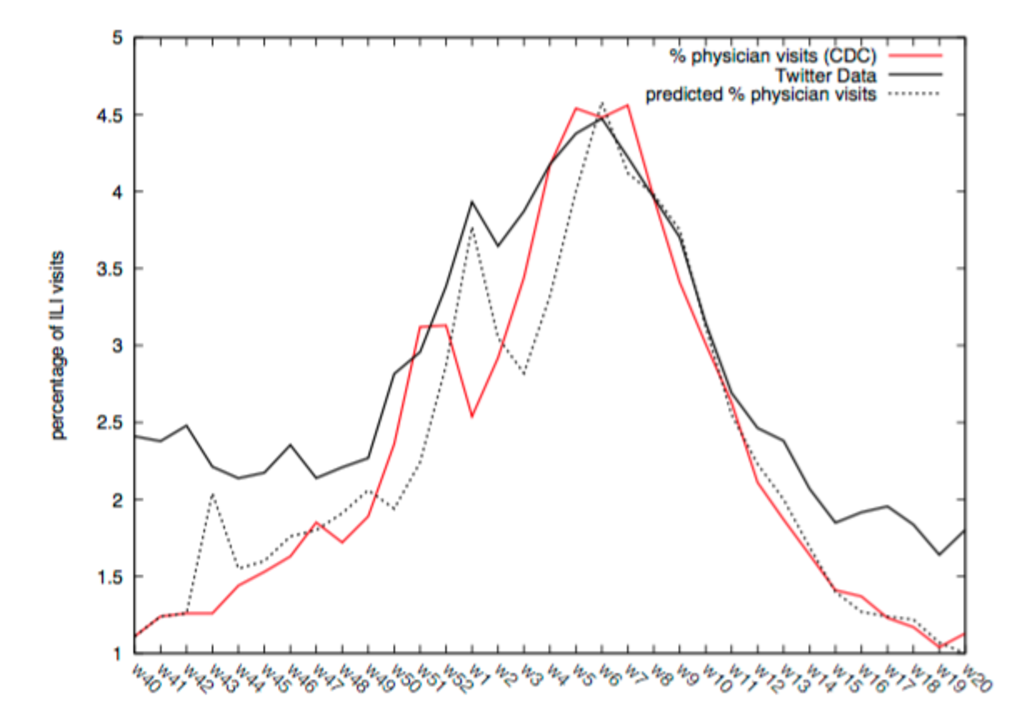
\includegraphics[width=0.5\textwidth]{images/Figure4.pdf}
  \caption{Weekly plot of percentage weighted ILI visits, positively classified Twitter
  dataset and predicted ILI rate using CDC and Twitter \cite{achrekar12}} 
  \label{fig:Figure4} 
\end{figure}


\subsection{Limitations of Using Search Queries and Social Media Data to Track Epidemics}

There is some evidence that influenza forecasting models based on Twitter data performed 
better than general search query data \cite{paul14}. Google Flu Trends (GFT) algorithms 
underestimated ILI in the U.S. at the start of the H1N1 (i.e. {\it swine flu}) pandemic 
in 2009 \cite{butler13}, and over-predicted seasonal influenza in January 2013 compared 
to the CDC ILI by almost double \cite{lazer14} (shown in Figure 5). As described above, 
there are important limitations in using social media data for predicting epidemics: 
First, internet access and Twitter usage is not uniform by geographical region. Urban areas 
have higher density of internet connections than rural areas \cite{yuan13}, and coastal 
regions of the U.S. (CA, NY) produced more tweets per person than Midwestern U.S. states 
(or Europe) \cite{achrekar12}. Thus, performance of seasonal influenza predictions models 
may be best applied to regions with high internet access and where tweets are more frequent. 
Second, exact demographic information about the Twitter population is not easy to estimate 
(or unknown) and the demographic of internet users does not represent characteristics of 
the general population.  Third, though promising, the results of this research are based 
on correlations between often noisy internet search queries or Twitter posts and physician 
reports of ILI compiled by official governmental sources. Caution should be  used in 
evaluating predictions about serious health concerns such as epidemics or pandemics 
based on correlational evidence as the data do not support causal inferences. 

\begin{figure}
  \centering
  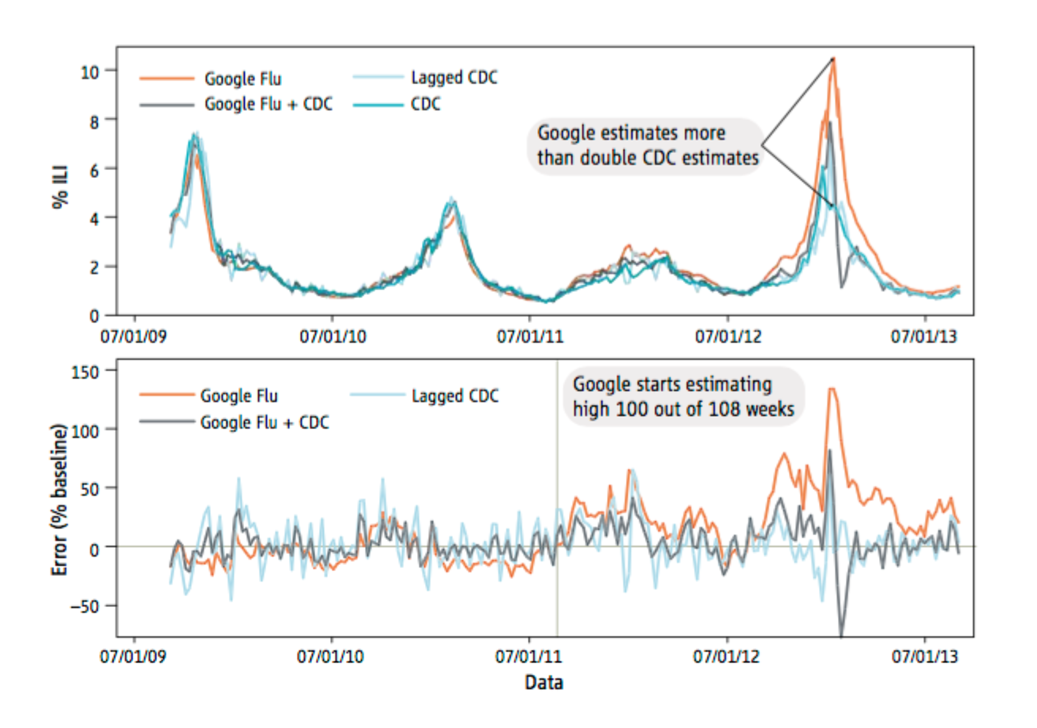
\includegraphics[width=0.5\textwidth]{images/Figure5.pdf}
  \caption{GFT overestimation: GFT overestimated the prevalence of flu in 2012-2013 season
  and overshot the actual level in 2011-2012 by more than 50 percent \cite{lazer14}} 
  \label{fig:Figure5} 
\end{figure}

\subsection{The Dynamics of Epidemic Spreading} 

Can these methods be extended to survey other types of epidemics? The dynamics of epidemic 
spreading is a complex phenomenon, based on contact networks of person-to-person interaction, 
indirect exposure, and transmission byways such as the {\it airline transportation network} 
(ATN) \cite{Colizza06}. Epidemics are quantified in terms of the proportion of the population 
infected, those yet to be infected, and the rate of transmission \cite{hethcote00}. In 
addition, the structure of the contact network can influence epidemic spreading 
\cite{pastor01}. For example, in the case of simple contagion, weak ties among acquaintances 
or infrequent associations provide shortcuts between distant nodes that reduce distance within 
the network \cite{granovetter73} and can facilitate the spread of disease. Furthermore, 
networks with ``small world'' properties have many nodes with few connections, but a small 
number of highly connected nodes that can rapidly transmit contagion throughout the network 
\cite{watts98}. Analyzing the correlation between Twitter posts and rate of ILI reports does 
not capture the complex network structure that underlies disease epidemics and pandemics. 
It is possible that by analyzing the structure of social media networks, future research 
may help to identify how points of connection within online networks are associated with 
the spread of contagion and resulting epidemics \cite{zhu17}. Some epidemics such as the
opioid crisis in North America \cite{volkow14} may be amenable to social network modeling
as drug usage, dependancy, and addiction is subserved by social networks. The emergence of 
new technologies, such as wearable biosensors \cite{carreiro15} may help improve geospatial 
mapping of the opioid epidemics and treatment interventions.

\section{Conclusion}

Big data mining of social media has tremendous potential to detect trends and confirm 
observations based on real time events, providing opportunities to monitor infectious 
disease on a global level. The research reviewed above shows how search queries and 
Twitter data about ILI related information provides an early detection signal that can
supplement existing epidemic monitoring systems and may help improve public health 
responses and prevention. As described above, these approaches to tracking disease and
predicting epidemics work best in areas with high internet connectivity and are better 
suited to populations with a high proportion of social media users.

\begin{acks}

  The author would like to thank Dr. Gregor von Laszewski for providing the LaTex template
  and instructions, many comments, helpful feedback, edits, and fixes. Thanks also 
  to the Assistant Instructors who were also very helpful in this learning process. 

\end{acks}

\bibliographystyle{ACM-Reference-Format}
\bibliography{report} 

\section{Bibtex Issues}
\todo[inline]{Warning--empty publisher in achrekar12}
\todo[inline]{Warning--empty address in achrekar12}
\todo[inline]{Warning--page numbers missing in both pages and numpages fields in achrekar12}
\todo[inline]{Warning--unrecognized DOI value [https://www.slideshare.net/hdachrekar/healthinf-2012]}
\todo[inline]{Warning--empty address in demchenko12}
\todo[inline]{Warning--unrecognized DOI value [doi:10.1038/nature07634]}
\todo[inline]{Warning--no number and no volume in gupta15}
\todo[inline]{Warning--page numbers missing in both pages and numpages fields in gupta15}
\todo[inline]{Warning--unrecognized DOI value [https://doi.org/10.1371/journal.pmed.1001413]}
\todo[inline]{Warning--page numbers missing in both pages and numpages fields in herland14}
\todo[inline]{Warning--unrecognized DOI value [https://doi.org/10.1186/2196-1115-1-2]}
\todo[inline]{Warning--unrecognized DOI value [https://doi.org/10.1137/S0036144500371907]}
\todo[inline]{Warning--empty publisher in lamb13}
\todo[inline]{Warning--empty address in lamb13}
\todo[inline]{Warning--require articleno with numpages field in pastor01}
\todo[inline]{Warning--page numbers missing in both pages and numpages fields in paul14}
\todo[inline]{Warning--unrecognized DOI value [https://doi.org/10.1371/journal.pone.0019467]}
\todo[inline]{Warning--unrecognized DOI value [https://doi.org/10.1371/journal.pone.0064323]}
\todo[inline]{Warning--require articleno with numpages field in zhu17}
\todo[inline]{(There were 19 warnings)}
\section{Issues}

\DONE{Example of done item: Once you fix an item, change TODO to DONE}

\subsection{Assignment Submission Issues}

    \DONE{Do not make changes to your paper during grading, when your repository should be frozen.}

\subsection{Uncaught Bibliography Errors}

    \DONE{Missing bibliography file generated by JabRef}
    \DONE{Bibtex labels cannot have any spaces, \_ or \& in it}
    \DONE{Citations in text showing as [?]: this means either your report.bib is not up-to-date or there is a spelling error in the label of the item you want to cite, either in report.bib or in report.tex}

\subsection{Formatting}

    \DONE{Incorrect number of keywords or HID and i523 not included in the keywords}
    \DONE{Other formatting issues}

\subsection{Writing Errors}

    \DONE{Errors in title, e.g. capitalization}
    \DONE{Spelling errors}
    \DONE{Are you using {\em a} and {\em the} properly?}
    \DONE{Do not use phrases such as {\em shown in the Figure below}. Instead, use {\em as shown in Figure 3}, when referring to the 3rd figure}
    \DONE{Do not use the word {\em I} instead use {\em we} even if you are the sole author}
    \DONE{Do not use the phrase {\em In this paper/report we show} instead use {\em We show}. It is not important if this is a paper or a report and does not need to be mentioned}
    \DONE{If you want to say {\em and} do not use {\em \&} but use the word {\em and}}
    \DONE{Use a space after . , : }
    \DONE{When using a section command, the section title is not written in all-caps as format does this for you}\begin{verbatim}\section{Introduction} and NOT \section{INTRODUCTION} \end{verbatim}

\subsection{Citation Issues and Plagiarism}

    \DONE{It is your responsibility to make sure no plagiarism occurs. The instructions and resources were given in the class}
    \DONE{Claims made without citations provided}
    \DONE{Need to paraphrase long quotations (whole sentences or longer)}
    \DONE{Need to quote directly cited material}

\subsection{Character Errors}

    \DONE{Erroneous use of quotation marks, i.e. use ``quotes'' , instead of " "}
    \DONE{To emphasize a word, use {\em emphasize} and not ``quote''}
    \DONE{When using the characters \& \# \% \_  put a backslash before them so that they show up correctly}
    \DONE{Pasting and copying from the Web often results in non-ASCII characters to be used in your text, please remove them and replace accordingly. This is the case for quotes, dashes and all the other special characters.}
    \DONE{If you see a figure and not a figure in text you copied from a text that has the fi combined as a single character}

\subsection{Structural Issues}

    \DONE{Acknowledgement section missing}
    \DONE{Incorrect README file}
    \DONE{In case of a class and if you do a multi-author paper, you need to add an appendix describing who did what in the paper}
    \DONE{The paper has less than 2 pages of text, i.e. excluding images, tables and figures}
    \DONE{The paper has more than 6 pages of text, i.e. excluding images, tables and figures}
    \DONE{Do not artificially inflate your paper if you are below the page limit}

\subsection{Details about the Figures and Tables}

    \DONE{Capitalization errors in referring to captions, e.g. Figure 1, Table 2}
    \DONE{Do use {\em label} and {\em ref} to automatically create figure numbers}
    \DONE{Wrong placement of figure caption. They should be on the bottom of the figure}
    \DONE{Wrong placement of table caption. They should be on the top of the table}
    \DONE{Images submitted incorrectly. They should be in native format, e.g. .graffle, .pptx, .png, .jpg}
    \DONE{Do not submit eps images. Instead, convert them to PDF}

    \DONE{The image files must be in a single directory named "images"}
    \DONE{In case there is a powerpoint in the submission, the image must be exported as PDF}
    \DONE{Make the figures large enough so we can read the details. If needed make the figure over two columns}
    \DONE{Do not worry about the figure placement if they are at a different location than you think. Figures are allowed to float. For this class, you should place all figures at the end of the report.}
    \DONE{In case you copied a figure from another paper you need to ask for copyright permission. In case of a class paper, you must include a reference to the original in the caption}
    \DONE{Remove any figure that is not referred to explicitly in the text (As shown in Figure ..)}
    \DONE{Do not use textwidth as a parameter for includegraphics}
    \DONE{Figures should be reasonably sized and often you just need to
  add columnwidth} e.g. \begin{verbatim}/includegraphics[width=\columnwidth]{images/myimage.pdf}\end{verbatim}

re
\end{document}
